\section{Background and Related work}\label{sec:rel}
%In this section, we survey previous work and focus on the most relevant pieces.
%Section~\ref{sec:trajvisana} and ~\ref{sec:interactive} summarize the related works in trajectory visual analysis and interactive data visualization for large dataset, respectively.

In this part, we survey related works on \textit{trajectory visualization methods} in Section~\ref{sec:trajvisana} and \textit{interactive data visualization for large datasets} in Section~\ref{sec:interactive}, respectively.

\subsection{Trajectory Visualization Methods}\label{sec:trajvisana}
A trajectory is a sequence of spatial locations (e.g., GPS positioning results) and trajectories are the most common representations of object movements. Existing trajectory visualization methods can be classified into three categories according to the form of visualization~\cite{chen2015survey}, i.e., \textit{point-based}, \textit{region-based}, and \textit{line-based}. We give a brief introduction to these methods and refer the interested readers to~\cite{chen2015survey} for more detailed discussions.


Point-based visualization plots the locations in the trajectories independently and captures the overall spatial distribution of the moving objects. Many density-based methods~\cite{liu2013vait,yang2016exploring,chae2014public,borruso2008network}, 
%~\cite{liu2013vait,yang2016exploring,chae2014public,xie2008kernel, borruso2008network}
e.g., kernel density estimation, are applied in point-based visualization to preserve the spatial distribution. Region-based visualization slices the entire region into sub-regions and visualizes the aggregated information in each sub-region~\cite{guo2009flow,von2015mobilitygraphs}.
%~\cite{guo2009flow,wood2010visualisation,von2015mobilitygraphs}
As region-based visualization focuses on aggregated statistics, it is most effective in capturing macro-patterns. In this work, we focus on line-based visualization, which uses polylines to connect the locations in each trajectory and shows the trace of object movements (see an example in Figure~\ref{fig:line}). As line-based visualization preserves the continuous movement information of objects~\cite{guo2011tripvista,hurter2009fromdady}, it is widely used in many visual analysis applications such as traffic management, urban planning, and route recommendation. However, line-based visualization is known to suffer from severe visual clutter, especially when the dataset is large. Several techniques have been proposed to alleviate visual clutter, such as clustering-based techniques~\cite{von2015mobilitygraphs}
%~\cite{ferreira2013vector, rinzivillo2008visually, von2015mobilitygraphs}
and advanced interaction techniques~\cite{ferreira2013visual}.
%~\cite{kruger2013trajectorylenses, ferreira2013visual}



\subsection{Interactive Visualization for Large Datasets}\label{sec:interactive}


Figure~\ref{fig:sys_framework} illustrates a general architecture of interactive visualization systems,
e.g., Spotfire\footnote{\url{https://www.tibco.com/products/tibco-spotfire}}, Tableau\footnote{\url{https://www.tableau.com/}}, ATLAS~\cite{chan2008maintaining}, Viate~\cite{yang2019vaite} and Marviq~\cite{dong2020marviq}.
There are typically three layers: user interface in the front-end layer, optimization techniques in the middle-layer, and database management system (usually cloud-based) in the back-end layer. The visualization community usually focuses on improving the effectiveness of data visualization at the front-end, e.g., designing novel visualization methods/toolkits such as D3\footnote{\url{https://d3js.org/}} to enable data analysts to effectively gain insights from data. 
The database community usually aims to improve query efficiency, e.g., devising big data systems such as Spark\footnote{\url{https://spark.apache.org/}} for efficient data processing at the back-end. 
With the popularization of location-acquisition devices, the scale of trajectory datasets can be extremely large. For example, the taxis in Shenzhen generate {$\sim$}9.3GB trajectory data per day. However, visualization generation has a long latency for large datasets due to heavy data processing/graphic rendering, which harms the responsiveness of interactive visualization. Therefore, both the visualization and database communities began to advance techniques in the middle-layer to reduce visualization latency for large datasets. We briefly elaborate these techniques as follows.


\begin{figure}
	\centering
	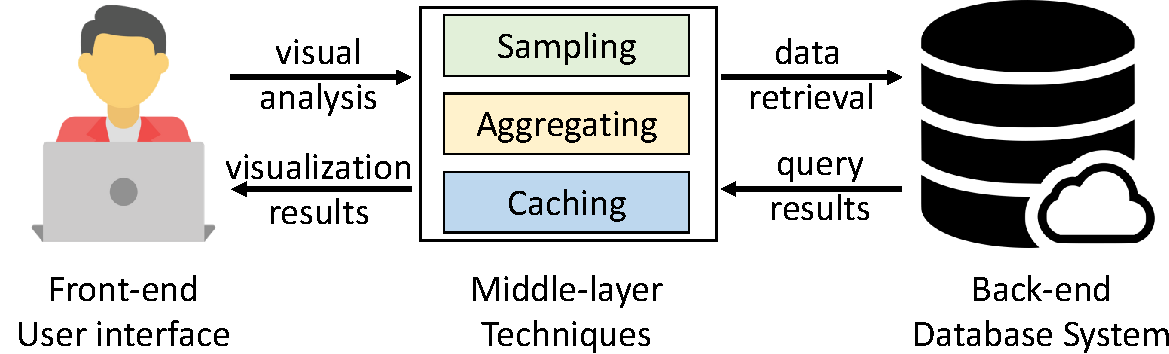
\includegraphics[width=0.36\textwidth]{pictures/framework/framework.pdf}
	\trim
	\caption{System architecture for interactive visualization.} \label{fig:sys_framework}
    \trim \trim
\end{figure}


\stitle{Aggregation-based techniques}
These works divide the {entire area} into basic units and visualize the aggregated information of the trajectories for each unit~\cite{wood2010visualisation,guo2009flow,von2015mobilitygraphs}. For more details on aggregation-based techniques, we refer the reader to~\cite{andrienko2008spatio,adrienko2010spatial}. Our problem and solutions are different from these works as we focus on visualizing the raw trajectories, instead of aggregated statistics.


\stitle{Sampling-based techniques} Sampling is widely used in both visualization and database communities ~\cite{battle2013dynamic,rapp2019void,chen2014visual,yu2020turbocharging,park2016visualization,qin2020making,DBLP:conf/sigmod/DingHCC016,DBLP:journals/pvldb/KimBPIMR15}. These works try to reduce the dataset to a subset with some special characteristics: such as blue noise property~\cite{rapp2019void}, multi-class property~\cite{chen2014visual} or maximize some user-defined quality~\cite{yu2020turbocharging}. The work most relevant to ours is~\cite{park2016visualization}, which is designed for scatter plots (a form of point-based visualization). It reduces the number of points in a plot while preserving the spatial distribution of the points in the original dataset. The techniques in~\cite{park2016visualization} cannot be applied to our trajectory visualization problem
as trajectory is more complex than individual scatter points (e.g., the order of GPS points is essential and the trajectories could have a large variance in length). Some works simplify a trajectory by sampling important points to reduce data size~\cite{zhang2018trajectory,2018arXiv180303550V} or alleviate visual clutter~\cite{borcan2012improving, 6851202}. These works are orthogonal to ours as we are sampling complete trajectories instead of points in a trajectory.

\stitle{Caching-based and other techniques}
Chan et al. propose ATLAS~\cite{chan2008maintaining}, which utilizes caching for efficient data communication between server and client.
ATLAS also exploits a powerful multi-core server to accelerate visual analysis tasks in both the middle-layer and back-end.
Piringer et al.~\cite{piringer2009multi} propose an architecture for interactive visual exploration,
which utilizes multi-core devices and avoids the common pitfalls of multi-threading to provide quick visual feedback.
Our work is orthogonal to these execution optimizations as we mainly focus on the algorithm perspective.

\sstitle{Novelties of our work} To the best of our knowledge, we are the first to formulate the quality optimal trajectory sampling problem to accelerate visualization on large scale datasets. We devise effective algorithms for this problem, which not only provide visual quality guarantee but also reduce the well-know visual clutter in trajectory visualization. Based on these algorithm, we design the $\avats$ framework with a tailored $\invQ$-tree index to produce high quality visualization for arbitrary target region with low latency.

